\chapter{Introduction}

Object Oriented Programming (OOP) languages have given programmers much freedom in expressing themselves in Object Oriented Design. However, they are still lacking in some areas when it comes to particular software design decisions such as cross-cutting concern.

Cross-cutting concerns are aspects of the program that scatter throughout different areas of the code base. These aspects cannot usually be separated easily or cleanly from the rest of the program. The essence of Aspect Oriented Programming~\cite{aop} is to find ways to solve the cross-cutting concern problems.

In this project, a framework called "Buffalo" is designed and implemented to solve this type of problem on the .NET platform. Buffalo makes use of the .NET attribute system to weave aspect code to any targeted methods. The design and rationale of the framework is discussed in Chapter 2. The implementation detail is given in Chapter 3.

The results indicate that by using Buffalo, developers can separate cross-cutting concerns from the core of the program for easy maintenance and ultimately be more productive. The analysis is discussed in Chapter 4.

The report concludes in Chapter 5 with the current project status. A set of planned future works is also discussed as well as what was learned from working on this project.

Buffalo comprises around 1,200 lines of source code. A user manual is included in Appendix A, which contains examples on how the system works. Instructions are also included for how to integrate Buffalo with MS-Build.


\section{Compiler Support}

There are several broad approaches to implementing an AOP framework. The ideal approach is to extend the compiler of the target language to provide built-in support, thus making AOP the first class citizen. However there are very few languages out there that take this approach; among the few are Delphi Prism~\cite{delphi_prism2010} and AspectJ~\cite{aspectj_faq, aspectj_text}. 

Microsoft is currently in the "wait and see" mode regarding support of AOP development in the C\# compiler~\cite{hejlsberg}. The alternative compiler, such as Mono C\#~\cite{monocsharp}, is open source, so technically, anyone can build AOP support into it. While that would have been a fun challenge, it would have been a fairly big undertaking, and there is concern that the project might not be finished in the time frame required.

That leaves framework support as the other viable option. There are several implementation techniques to provide AOP capabilities~\cite{aopcs, postsharp, aspectcs} via framework.

\section{Run-time Interception}

Early on the implementation, approaches were narrowed down to two approaches: Run-time Interception and Post Compilation Weaving. As its name suggested, Run-time Interception operates while the program is in execution. It uses the proxy pattern where client communicates with the target object via a proxy, and aspects are injected to the proxy. This enables run-time behavior of the program to be modified. Figure~\ref{proxy_model} illustrates this process.

\begin{figure}[H]
  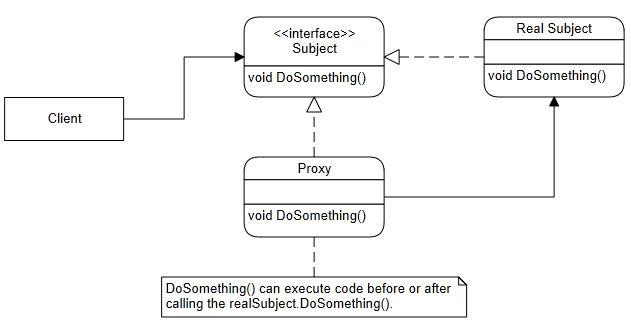
\includegraphics[scale=1.0]{Proxy3.PNG}
  \centering
  \caption{AOP Framework Using Proxy Pattern\label{proxy_model}}
\end{figure}

New functionality can be “added” to the target object via the proxy. The disadvantage of this approach is that it involves the generation of proxy object at run-time. As a result, the run-time performance of the application will be impacted. It is also restricting in that both target object and the proxy must implement a common interface for this to work and that only virtual methods are exposed for interception.

From the end user's perspective, to use it, the developer usually must provide some type of mapping between the target object and the proxy via a configuration file so that the actual proxy generation can occur. 

Although this approach is easier to implement, it is not as easy and user-friendly. Buffalo is not taking this approach mainly because one of the goals is to keep it flexible and simple to use.

\section{Post Compilation Weaving}

The approach Buffalo takes is Post Compilation Weaving. The idea is that after compilation of the source code, Buffalo takes over to disassemble the assembly and weaves in the defined aspect code to all targeted methods. This approach is more difficult to implement as it involves modifying the underlying assembly by changing Common Intermediate Language (CIL) instructions~\cite{rewrite_msil}. However, the advantage is that no run-time performance of proxy generation will be needed. Therefore, no messy configuration is required.

Since injection happens post-compilation, the whole process can be integrated into the MS-Build system to have the weaving invoked automatically if needed. This will further reduce the steps needed from the developer.

Figure~\ref{buffalo_model} shows an overview of the compilation process and where Buffalo will fit in the process.

\begin{figure}[H]
  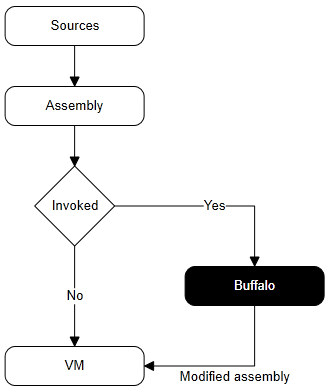
\includegraphics[scale=1.0]{BuffaloOverview2.PNG}
  \centering
  \caption{Buffalo Model\label{buffalo_model}}
\end{figure}


